\documentclass{article}

% Language setting
% Replace `english' with e.g. `spanish' to change the document language
\usepackage[english]{babel}

% Set page size and margins
% Replace `letterpaper' with`a4paper' for UK/EU standard size
\usepackage[letterpaper,top=2cm,bottom=2cm,left=3cm,right=3cm,marginparwidth=1.75cm]{geometry}

% Formatting
\usepackage{blindtext}
\usepackage[T1]{fontenc}
\usepackage[utf8]{inputenc}
\usepackage[margin=1in]{geometry}

% Useful packages
\usepackage{amsmath}
\usepackage{graphicx}
\usepackage[colorlinks=true, allcolors=blue]{hyperref}
\usepackage{minted}
\title{Artificial intelligence - Project 3 \\ - Limbaje de planificare -}
\author{Pop Ruxandra Maria, Zelenszky Bianca}
\date{14/01/2022}

\begin{document}
\maketitle

\thispagestyle{empty}
 \section{Introducere}

Pentru realizarea acestui proiect au fost nevoie de cunostințe legate de planificarea unei probleme și găsirea pașilor care duc la un scop bine stabilit.
Astfel am folosit limbajul PDDL, care generează toate stările unei probleme, ce are un domeniu unic.
\\ 

Componentele unei sarcini de planificare în PDDL sunt:
 \begin{itemize}
    \setlength\itemsep{0em}
    \item Objects = lucruri din lumea reală care ne interesează
    
    \item  Predicates = proprietăți ale obiectelor care ne interesează
    \item Initial state  = starea lumii în care începem
    \item Goal specification = lucruri care vrem să fie adevărate
    \item Actions/Operators =  modalități de schimbare a stării lumii
\end{itemize}

O problemă de planificare este creată prin asocierea unei descrieri de domeniu cu o descriere a problemei. Condițiile pre și post ale acțiunii sunt exprimate ca propoziții logice construite din predicate și termeni de argumente și conectivități logice.
\newline
\newline
Sarcinile de planificare specificate în PDDL sunt separate în două fișiere diferite:

 \begin{itemize}
    \setlength\itemsep{0em}
    \item Fișier de domeniu care conține predicatele și acțiunile
       \item Fișier cu probleme care conține obiectele, starea inițială și specificația goal-ului
    
\end{itemize}

Structura fișierului de domeniu este următoarea:
\bigskip
\\

(define (domain <domain  name> )

 (:predicates <predicate>)

         (:action  <prima actiune>)
      
         .......................
      
         (:action  <ultima actiune>)
)

\bigskip

Structura fișierului de probleme este următoarea:
\bigskip
\\

(define (problem <problem name>)

        (:domain <domain name>)
        
        (:objects  <obiecte>)
    
        (:init <starea initiala>)
     
        (:goal <starea finala>)
)
\section{Cerința problemei}
Am ales să implementam două tipuri de domenii, unul cu aplicabilitate în lumea reala, și unul fără.
Fiecare domeniu are ca scop realizarea unei rețete. Astfel, prima problemă are ca și scop final realizarea unei prăjituri cu măr, iar cea de a doua are ca scop realizarea unei pizza.

Realizarea unei rețete necesită urmarea unor pași cum ar fi: cumpărarea ingredientelor necesare, realizarea compoziției.

 Problemele definite de domeniul cu aplicabilitate în lumea reală prezintă o stare inițiala parțial definită, acțiunile având efecte nedeterministe, și anume nu știm dacă un anume ingredient e stricat sau nu, urmând ca programul să determine care ingredient e stricat și care nu.
 
 \newline
 Problemele fără aplicabilitate în lumea reală nu întâlnesc aceste situații ale  mediului parțial observabil, aici fiind foarte clar care ingrediente sunt stricate și care nu.
 
 
\newline





\begin{center}
\begin{figure}[htb]
 \centering 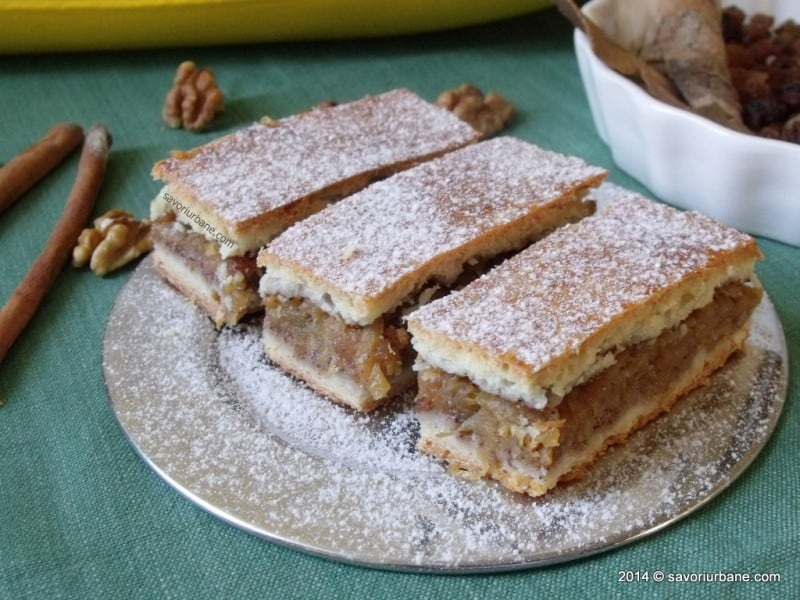
\includegraphics[width=50mm,scale=0.5]{prajitura.jpeg}
 \caption{Goal-ul pentru problema 1.}
  \label{fig:boat1}
  \end{figure}
\end {center}
\begin{figure}[htb]
 \centering 
\includegraphics[width=50mm,scale=0.5]{pizza.jpeg}
 \caption{Goal-ul pentru problema 2.}
  \label{fig:boat2}
  \end{figure}


\newpage
 \section{Implementare}

Pentru realizarea acestor cerințe este nevoie de a defini domeniul și diferite probleme. Domeniul descriind cum arata mediul în care se desfășoară acțiunile, obiectele (agenții) care fac acțiunile și acțiunile care se petrec în acest mediu. Având un domeniu stabilit, se pot genera diferite probleme pe baza lui. În probleme se folosesc obiectele și acțiunile declarate în domeniu, după care se urmarește crearea unei condiții inițiale din care să rezulte o anumită stare finală  definită de noi.

Ambele probleme create de noi au aceeași idee de implemetare, diferentă fiind faptul că una are aplicabilitate în mediul real, iar alta nu.
\newline

\newline
\subsection{Problema fară aplicabilitate în lumea reală}
\subsubsection{Reprezentare domeniu pentru rețetă}
Predicatele domeniului sunt:
 \begin{itemize}
    \setlength\itemsep{0em}
    \item nu are i1 ?i1: nu are ingredientul 1
    \item nu are i2 ?i2: nu are ingredientul 2
    \item nu are i3 ?i3: nu are ingredientul 3
    \item nu are i4 ?i4: nu are ingredientul 4
    \item nu preparat final ?fin: preparatul final nu e gata
    \item neincalzit ?c: cuptorul nu este încalzit
    \item nu are amestec ? a: amestecul pentru rețetă nu e gata
    \item nu in cuptor ?c ?a: amestecul nu este băgat în cuptor
    \item nu gata ?fin:  rețeta nu e gata
  


\end{itemize}
Funcțiile domeniului sunt:

 \begin{itemize}
    \setlength\itemsep{0em}
    \item calitate-i1 ?i1: returnează calitatea ingredientului 1
    \item calitate-i2 ?i2: returnează calitatea ingredientului 2
    \item calitate-i3 ?i3: returnează calitatea ingredientului 3
    \item calitate-i4 ?i4: returnează calitatea ingredientului 4
    \item total-cost: calculează costul total


\end{itemize}
Acțiunile domeniului sunt:

 \begin{itemize}
    \setlength\itemsep{0em}
    \item cumparare ingredient1: cumpără primul ingredient
    \item cumparare ingredient2: cumpără al doilea ingredient
    \item cumparare ingredient3: cumpără al treilea ingredient
    \item cumparare ingredient4: cumpăra al patrulea ingredient
    \item start reteta: aici începe să se prepare rețeta
    \item amestec ingrediente:  amestecă ingredientele pentru a obține aluatul
    \item incalzire cuptor: încalzeste cuptorul pentru a adăuga aluatul
    \item  gata final: preparatul este gata și pregătit pentru servire
    
\end{itemize}





\textbf{Code:}
% a se completa fisierul code/dfs.py

    \inputminted[linenos]{C}{cod/domain_reteta_heuristics.pddl}
\bigskip
\textbf{ Explicații:}

  \begin{itemize}
    \setlength\itemsep{0em}
    \item La linia 3, pentru generalitate, în loc să specificăm un anumit tip de ingredient (de exemplu ouă sau brânză), am declarat
  tipul ingredientX, X fiind de la 1 la 4. Asta înseamnă că, pentru acest domeniu, avem nevoie obligatoriu de un număr de 4 
  ingrediente pentru a realiza rețeta. De asemenea, final și amestec au fost puse tot pentru generalitate (în problemă, tipul 
  final se referă la pizza, prăjitură etc., iar amestec la aluat, pastă etc.). 
    \item 	La liniile 16-22 sunt functiile domeniului. Avem o funcție de calitate pentru fiecare ingredient și funcția total-cost pe care
  îl folosim pentru selectarea produselor ce vor fi cumpărate.
    \item 	La liniile 25-52 are loc cumpărarea ingredientelor. Aici crește totodată și costul total în funcție de calitatea fiecărui 
  produs. Ingredientele vor fi alese în funcție de euristici.
    \item La liniile 55-66 este acțiunea start reteta. Aceasta incepe prepararea produsului final doar dacă are toate ingredientele la 
  îndemână.
    \item La liniile 68-84 este acțiunea amestec ingrediente. Aici se consumă ingredientele pentru a obține un amestec.
    \item La liniile 86-102 are loc acțiunea incalzire cuptor. Aici, amestecul se pune în cuptor și se încălzește
    \item La liniile 104-117 are loc acțiunea gata final, unde se scoate amestecul din cuptor, și se generează produsul final.
  
\end{itemize}


\bigskip
    



 \begin{itemize}
    \setlength\itemsep{0em}
 


\end{itemize}


\textbf{Comanda pentru rularea codului din terminal:}
prover9 -f ”aut.in”
\subsubsection{Reprezentare problema 1}
Prima problemă reprezintă realizarea unei rețete pentru o prajitură cu măr.
Obiectele problemei sunt:

 \begin{itemize}
    \setlength\itemsep{0em}
    \item ou1, ou2, ou3, ou4: reprezintă primul ingredient
    \item mar1, mar2, mar3: reprezintă al doilea ingredient
    \item lapte1, lapte2: reprezintă al treilea ingredient
    \item faina: reprezintă al patrulea ingredient
    \item prajitura: reprezintă produsul care trebuie să rezulte în urma realizării rețetei
    \item cuptor: reprezintă cuptorul unde va fi adăugat aluatul pentru prăjitură
    \item aluat: reprezintă aluatul format în urma amestecării tuturor ingredientelor


\end{itemize}
\textbf{Code:}
% a se completa fisierul code/dfs.py

    \inputminted[linenos]{C}{cod/problem_reteta_heuristics.pddl}
    
 \textbf{ Explicații:}

  \begin{itemize}
    \setlength\itemsep{0em}
    \item Liniile 13-47 reprezintă starea inițială a problemei. În această stare, o personă nu are nici un ingredient la dispoziție, cuptorul este neîncalzit, iar prajitura nu e gata
    \item Liniile 32-45 prezintă calitatea ingredientelor cumpărate. Un ingredient e de calitate dacă numărul asociat lui este cât
  mai mic. De exemplu, mărul 3 din magazin (calitate = 4) este mai bun decât mărul 1 (calitate = 10). Acest lucru este 
  important deoarece, precum se vede la linia 66, pe lângă scopul de a se face prăjitura, aceasta trebuie să fie
  cea mai bună, adică să fie formată din ingredientele cele mai bune (suma ingredientelor să fie minimă).  
  \item Linia 51 reprezintă scopul problemei, adică să fie gata prajitura (evidențiat prin predicatul negat (not (nu gata 
  prajitura).

  
\end{itemize}   

\newpage

\subsubsection{Reprezentare problema 2}
A doua  problemă reprezintă realizarea unei rețete pentru o pizza.
Obiectele problemei sunt:

 \begin{itemize}
    \setlength\itemsep{0em}
    \item branza1, branza2: reprezintă primul ingredient
    \item masiline1, masline2, masline3, masline4: reprezintă al doilea ingredient
    \item salam: reprezintă al treilea ingredient
    \item ciuperci: reprezintă al patrulea ingredient
    \item pizza: reprezintă produsul care trebuie să rezulte în urma realizării rețetei
    \item cuptor: reprezintă cuptorul unde va fi adăugat aluatul pentru pizza
    \item aluat: reprezintă aluatul format în urma amestecării tuturor ingredientelor


\end{itemize}
\textbf{Code:}
% a se completa fisierul code/dfs.py

    \inputminted[linenos]{C}{cod/problem2_reteta_heuristics.pddl}
    
 \textbf{ Explicații:}

  \begin{itemize}
    \setlength\itemsep{0em}
    \item Această problema e asemanatoare cu cea de la problema reteta heuristics, numai că în acest caz am ales să urmăm rețeta pentru o pizza, deci avem alte ingrediente și alte valori de calitate.

  
\end{itemize}   
    
    
    
    
    
    
    
    
    
    
\newpage





\subsection{Problema cu aplicabilitate în lumea reala}
\subsubsection{Reprezentare domeniu pentru rețetă}

Predicatele domeniului sunt:
 \begin{itemize}
    \setlength\itemsep{0em}
    \item nu are i1 ?i1: nu are ingredientul 1
    \item nu are i2 ?i2: nu are ingredientul 2
    \item nu are i3 ?i3: nu are ingredientul 3
    \item nu are i4 ?i4: nu are ingredientul 4
    \item stricat i1 ?1: ingredientul 1 e stricat
      \item stricat i2 ?2: ingredientul 2 e stricat
        \item stricat i3 ?3: ingredientul 3 e stricat
       
    \item nu preparat final ?fin: preparatul final nu e gata
    \item neincalzit ?c: cuptorul nu este încălzit
    \item nu are amestec ? a: amestecul pentru rețetă nu e gata
    \item nu in cuptor ?c ?a: amestecul nu este băgat în cuptor
    \item nu gata ?fin: rețeta nu e gata
  


\end{itemize}
Acțiunile domeniului sunt:

 \begin{itemize}
    \setlength\itemsep{0em}
    \item sense stricat i1: verifică dacă ingredientul 1 e stricat
        \item sense stricat i2: verifică dacă ingredientul 2 e stricat
            \item sense stricat i3: verifică dacă ingredientul 3 e stricat
    \item cumparare ingredient1: cumpără primul ingredient
    \item cumparare ingredient2: cumpără al doilea ingredient
    \item cumparare ingredient3: cumpără al treilea ingredient
    \item cumparare ingredient4: cumpără al patrulea ingredient
    \item arunc i1 stricat: dacă ingredientul 1 e stricat, se aruncă
       \item arunc i2 stricat: dacă ingredientul 2 e stricat, se aruncă
          \item arunc i3 stricat: dacă ingredientul 3 e stricat, se aruncă
    \item start retea: aici începe să se prepare produsul
    \item amestec ingrediente: amestecă ingredientele pentru a obține aluatul
    \item incalzire cuptor: încălzește cuptorul pentru a adăuga aluatul
    \item  gata final: preparatul este gata și pregătit pentru servire
    
\end{itemize}


\textbf{Code:}
% a se completa fisierul code/dfs.py

    \inputminted[linenos]{C}{cod/domain_reteta_contingent.pddl}


\textbf{ Explicații:}
    
  \begin{itemize}
    \setlength\itemsep{0em}
    \item La liniile 9-11 se remarcă 3 predicate care anunță dacă un ingredient e stricat. Asta înseamnă că pentru o problemă, numărul 
  maxim de ingrediente care pot să fie stricate este 3 (una pentru fiecare tip de ingredient, în afară de unul singur).
    \item La liniile 19-37 se observă elementul predicatul necunoscut stricat ingredient pentru a testa dacă are trebuie aruncat sau nu.
  îl folosim pentru selectarea produselor ce vor fi cumpărate. De asemenea, precondiția pentru a începe observarea este să fi cumpărat ingredientul.
    \item 	La liniile 63-82 are loc acțiunea de aruncare a ingredientelor dacă sunt stricate. După efectuarea acțiunii, se pierde ingredientul
  și trebuie cumpărat altul.
    \item La liniile 86-99, acțiunea start reteta, pe lângă faptul că trebuie să aibă câte una din fiecare tip de ingredient la dispoziție, 
  acestea nu trebuie să fie stricate.  
    \item La liniile 101-117 este acțiunea amestec ingrediente. Aici se consumă ingredientele pentru a obține un amestec.
    \item La liniile 119-135 are loc acțiunea incalzire cuptor. Aici, amestecul se pune în cuptor și se încălzește
    \item La  liniile 137-150 are loc acțiunea gata final, unde se scoate amestecul din cuptor, și se generează produsul final.
  
\end{itemize}


\newpage

\subsubsection{Reprezentare problema 1}
Prima problema reprezintă realizarea unei rețete pentru o prăjitură cu măr.
Obiectele problemei sunt:

 \begin{itemize}
    \setlength\itemsep{0em}
    \item ou1, ou2, ou3, ou4: reprezintă primul ingredient
    \item mar1, mar2, mar3: reprezintă al doilea ingredient
    \item lapte1, lapte2: reprezintă al treilea ingredient
    \item faina: reprezintă al patrulea ingredient
    \item prajitura: reprezintă produsul care trebuie să rezulte în urma realizării rețetei
    \item cuptor: reprezintă cuptorul unde va fi adaugat aluatul pentru prajitură
    \item aluat: reprezintă aluatul format în urma amestecării tuturor ingredientelor


\end{itemize}

% a se completa fisierul code/dfs.py

    \inputminted[linenos]{C}{cod/problem_reteta_contingent.pddl}
    
 \textbf{ Explicații:}

  \begin{itemize}
    \setlength\itemsep{0em}
    \item La liniile 32-43 am implementat ideea că un ingredient de un anumit tip din totalul de ingrediente din acel tip e stricat 
  (de exemplu, unul din cele 4 ouă sunt stricate, sau un măr din cele 3 e stricat). 
    \item La liniile 52-61 din scop, am evidențiat faptul că trebuie consumate toate ingredientele. Acest lucru evită situația de a
  cumpăra toate produsele din prima, și apoi să nu aibă loc acțiunea de arunc ingredient stricat (pentru ca nu ar mai avea rost).
 

  
\end{itemize}   


\subsubsection{Reprezentare problema 2}
A doua problemă reprezintă realizarea unei rețete pentru o pizza.
Obiectele problemei sunt:

 \begin{itemize}
    \setlength\itemsep{0em}
    \item branza1, branza2: reprezintă primul ingredient
    \item masiline1, masline2, masline3, masline4: reprezintă al doilea ingredient
    \item salam: reprezintă al treilea ingredient
    \item ciuperci: reprezintă al patrulea ingredient
    \item pizza: reprezintă produsul care trebuie să rezulte în urma realizării rețetei
    \item cuptor: reprezintă cuptorul unde va fi adăugat aluatul pentru pizza
    \item aluat: reprezintă aluatul format în urma amestecării tuturor ingredientelor


\end{itemize}
\textbf{Code:}
% a se completa fisierul code/dfs.py

    \inputminted[linenos]{C}{cod/problem2_reteta_contingent.pddl}
    
 \textbf{ Explicații:}

  \begin{itemize}
    \setlength\itemsep{0em}
    \item Această problemă e asemănătoare cu cea de la problem reteta contingent, numai că în acest caz am ales urmăm rețeta pentru o
  pizza, deci avem alte ingrediente și 2 tipuri de ingrediente stricate.

  
\end{itemize}   
    
    
 \section{Rezultate}
 
 \subsection{Intersecție nedirijată}
 \textbf{Demonstrație:}
 
 Pentru a ilustra corectitudinea acestui cod, vom începe prin a demonstra un caz particular: cel în care goal-ul este trace3(M4). Asta înseamnă că mașina M4 este a treia care trece în intersecție.
 	Se știe că:
 	
 	 \begin{itemize}
    \setlength\itemsep{0em}
    \item Mașina M1 nu semnalizează. Rezultă că M1 nu semnalizează nici la stânga, nici la dreapta, deci merge în față.  (1)
    \item Mașina M2 semnalizează dreapta. Rezultă că M2 merge la dreapta și are prima dată prioritate. (2)
    \item Mașina M4 nu semnalizează. Analog cu (1), M4 merge în față. (3)
    \item În dreapta lui M1 se află M2. (4)
    \item În dreapta lui M4 se află M1. (5)
    \item Prioritatea este unică (nu poți avea două mașini cu aceeași prioritate). (6)
    \item Într-o intersecție nedirijată se aplică prioritatea de dreapta. (7)
\end{itemize}

Din (7) rezultă că următoarea mașină care o să aibă prioritate o să fie mașina care are în dreapta mașina care a avut prima dată prioritate (2) și care merge în față (1). Deci va trece mașina M1 (4) și M1 devine prioritar pentru restul mașinilor (8) (deoarece M2 a trecut și (6)).

Din (7) rezultă că următoarea mașină care o să aibă prioritate o să fie mașina care are în dreapta mașina care a avut a doua oară prioritate (8) și care merge în față (3). Deci va trece mașina M4 (5) (deoarece M2 și M1 au trecut și (6)).

	Astfel, am demonstrat că a treia mașină care trece este M4.
	
	
\textbf{Code:}
% a se completa fisierul code/dfs.py

    \inputminted[linenos]{C}{cod/aut.out}	
 \subsection{Intersecție dirijată}
 
 Pentru a ilustra corectitudinea acestui cod, vom începe prin a demonstra un caz particular: cel în care goal-ul este trace3(M3). Asta înseamnă că mașina M3 este a treia care trece în intersecție. Se știe că:
 
\begin{itemize}
    \setlength\itemsep{0em}
    \item Mașina M1 semnalizează la stânga. Rezultă că M1 merge la stânga. (1)
    \item Mașina M2 nu semnalizează. Rezultă că M2 nu semnalizează nici la stânga, nici la dreapta, deci merge în față. (2)
    \item Mașina M3 nu semnalizează. Analog cu (2), M3 merge în față. (3)
    \item Mașina M4 semnalizează la stânga. Rezultă că M1 merge la stânga. (4)
    \item Semnul de la intrarea în intersecție a lui M1 este de cedează trecerea. (5)
    \item Semnul de la intrarea în intersecție a lui M2 este de drum cu prioritate. (6)
    \item Semnul de la intrarea în intersecție a lui M3 este stop. (7)
    \item Semnul de la intrarea în intersecție a lui M4 este de drum cu prioritate. (8)
    \item Prima dată trec mașinile de pe drumul cu prioritate (9)
    
\end{itemize}

Din (6) și (8) rezultă că mașinile M2 și M4 sunt pe aceeasi stradă cu prioritate. (10)

Din (5) și (7) rezultă că mașinile M1 și M3 sunt pe aceeași stradă fără prioritate. (11)

Din (9), (10), faptul că mașina M2 merge in față (2) și mașina M4 merge la stânga (4), rezultă că M2 are prioritate și trece primul, iar M4 trece al doilea.

Din (9), (11), faptul că mașina M3 merge în față (3) și mașina M1 merge la stânga (1), rezultă că M3 trece al treilea și M1 ultimul. 

Astfel, am demonstrat că a treia mașină care trece este M3.

\textbf{Code:}
% a se completa fisierul code/dfs.py

    \inputminted[linenos]{C}{cod/aut_dir.out}	
 \section{Concluzie}
 
În concluzie, acest proiect ne-a ajutat să ne aprofundăm cunoștințele acumulate pe parcursul laboratoarelor. Am  învățat să dezvoltam și să planificăm probleme ce necesită o parte logică. Totodata am învățat să scriem cod în limbajul PDDL.
% \section{Introduction}

% Your introduction goes here! Simply start writing your document and use the Recompile button to view the updated PDF preview. Examples of commonly used commands and features are listed below, to help you get started.

% Once you're familiar with the editor, you can find various project setting in the Overleaf menu, accessed via the button in the very top left of the editor. To view tutorials, user guides, and further documentation, please visit our \href{https://www.overleaf.com/learn}{help library}, or head to our plans page to \href{https://www.overleaf.com/user/subscription/plans}{choose your plan}.

% \section{Some examples to get started}

% \subsection{How to create Sections and Subsections}

% Simply use the section and subsection commands, as in this example document! With Overleaf, all the formatting and numbering is handled automatically according to the template you've chosen. If you're using Rich Text mode, you can also create new section and subsections via the buttons in the editor toolbar.

% \subsection{How to include Figures}

% First you have to upload the image file from your computer using the upload link in the file-tree menu. Then use the includegraphics command to include it in your document. Use the figure environment and the caption command to add a number and a caption to your figure. See the code for Figure \ref{fig:frog} in this section for an example.

% Note that your figure will automatically be placed in the most appropriate place for it, given the surrounding text and taking into account other figures or tables that may be close by. You can find out more about adding images to your documents in this help article on \href{https://www.overleaf.com/learn/how-to/Including_images_on_Overleaf}{including images on Overleaf}.

% \begin{figure}
% \centering
% \includegraphics[width=0.3\textwidth]{frog.jpg}
% \caption{\label{fig:frog}This frog was uploaded via the file-tree menu.}
% \end{figure}

% \subsection{How to add Tables}

% Use the table and tabular environments for basic tables --- see Table~\ref{tab:widgets}, for example. For more information, please see this help article on \href{https://www.overleaf.com/learn/latex/tables}{tables}. 

% \begin{table}
% \centering
% \begin{tabular}{l|r}
% Item & Quantity \\\hline
% Widgets & 42 \\
% Gadgets & 13
% \end{tabular}
% \caption{\label{tab:widgets}An example table.}
% \end{table}

% \subsection{How to add Comments and Track Changes}

% Comments can be added to your project by highlighting some text and clicking ``Add comment'' in the top right of the editor pane. To view existing comments, click on the Review menu in the toolbar above. To reply to a comment, click on the Reply button in the lower right corner of the comment. You can close the Review pane by clicking its name on the toolbar when you're done reviewing for the time being.

% Track changes are available on all our \href{https://www.overleaf.com/user/subscription/plans}{premium plans}, and can be toggled on or off using the option at the top of the Review pane. Track changes allow you to keep track of every change made to the document, along with the person making the change. 

% \subsection{How to add Lists}

% You can make lists with automatic numbering \dots

% \begin{enumerate}
% \item Like this,
% \item and like this.
% \end{enumerate}
% \dots or bullet points \dots
% \begin{itemize}
% \item Like this,
% \item and like this.
% \end{itemize}

% \subsection{How to write Mathematics}

% \LaTeX{} is great at typesetting mathematics. Let $X_1, X_2, \ldots, X_n$ be a sequence of independent and identically distributed random variables with $\text{E}[X_i] = \mu$ and $\text{Var}[X_i] = \sigma^2 < \infty$, and let
% \[S_n = \frac{X_1 + X_2 + \cdots + X_n}{n}
%       = \frac{1}{n}\sum_{i}^{n} X_i\]
% denote their mean. Then as $n$ approaches infinity, the random variables $\sqrt{n}(S_n - \mu)$ converge in distribution to a normal $\mathcal{N}(0, \sigma^2)$.


% \subsection{How to change the margins and paper size}

% Usually the template you're using will have the page margins and paper size set correctly for that use-case. For example, if you're using a journal article template provided by the journal publisher, that template will be formatted according to their requirements. In these cases, it's best not to alter the margins directly.

% If however you're using a more general template, such as this one, and would like to alter the margins, a common way to do so is via the geometry package. You can find the geometry package loaded in the preamble at the top of this example file, and if you'd like to learn more about how to adjust the settings, please visit this help article on \href{https://www.overleaf.com/learn/latex/page_size_and_margins}{page size and margins}.

% \subsection{How to change the document language and spell check settings}

% Overleaf supports many different languages, including multiple different languages within one document. 

% To configure the document language, simply edit the option provided to the babel package in the preamble at the top of this example project. To learn more about the different options, please visit this help article on \href{https://www.overleaf.com/learn/latex/International_language_support}{international language support}.

% To change the spell check language, simply open the Overleaf menu at the top left of the editor window, scroll down to the spell check setting, and adjust accordingly.

% \subsection{How to add Citations and a References List}

% You can simply upload a \verb|.bib| file containing your BibTeX entries, created with a tool such as JabRef. You can then cite entries from it, like this: \cite{greenwade93}. Just remember to specify a bibliography style, as well as the filename of the \verb|.bib|. You can find a \href{https://www.overleaf.com/help/97-how-to-include-a-bibliography-using-bibtex}{video tutorial here} to learn more about BibTeX.

% If you have an \href{https://www.overleaf.com/user/subscription/plans}{upgraded account}, you can also import your Mendeley or Zotero library directly as a \verb|.bib| file, via the upload menu in the file-tree.

% \subsection{Good luck!}

% We hope you find Overleaf useful, and do take a look at our \href{https://www.overleaf.com/learn}{help library} for more tutorials and user guides! Please also let us know if you have any feedback using the Contact Us link at the bottom of the Overleaf menu --- or use the contact form at \url{https://www.overleaf.com/contact}.

% \bibliographystyle{alpha}
% \bibliography{sample}

\end{document}